% Intended LaTeX compiler: pdflatex
\documentclass[10pt,a4paper,UTF8]{article}
\usepackage{zclorg}
\author{zcl.space}
\date{}
\title{通信系统中的随机过程}
\hypersetup{
 pdfauthor={zcl.space},
 pdftitle={通信系统中的随机过程},
 pdfkeywords={},
 pdfsubject={},
 pdfcreator={Emacs 25.0.50.1 (Org mode 9.0.5)}, 
 pdflang={English}}
\begin{document}

\maketitle
在 \href{one-dimension-random-walk.org}{一维随机游动} 的例子中,我们讨论了参数离散取值离散的随机过程,今天,给出一个参数连续取值离散的随机过程。

\begin{problem}
设有一个脉冲数字通信系统,它传送的信号是脉冲宽度为\(T_{0}\)的脉冲信号,每隔\(T_{0}\)送出一个脉冲。脉冲幅度\(\xi(t)\)是一个随机变量,它可取四个值\(\{-2,-1,1,2\}\),且取这四个值的概率是相同的,即:
\begin{eqnarray*}
P(\xi(t) = 2)&=&P(\xi(t) = 1) \\
&=&P(\xi(t) = -1) \\
&=&P(\xi(t) = -2) \\
&=&1/4
\end{eqnarray*}

不同周期内脉冲幅度是相互统计独立的,脉冲的起始时间相对于原点\(t=0\)的时间差\(u\)为均匀分布在\(0,T_{0}\)内的随机变量。试求在两个时刻\(t_{1},t_{2}\)该随机过程\(\xi(t)\)所取值\(\xi(t_{1}),\xi(t_{2})\)的二维联合概率密度。
\end{problem}

\begin{answer}
首先,给出一个该脉冲数字通信数字信号的一个典型样本函数。如图\ref{fig:orga4a4c7f}所示
\begin{figure}[htbp]
\centering
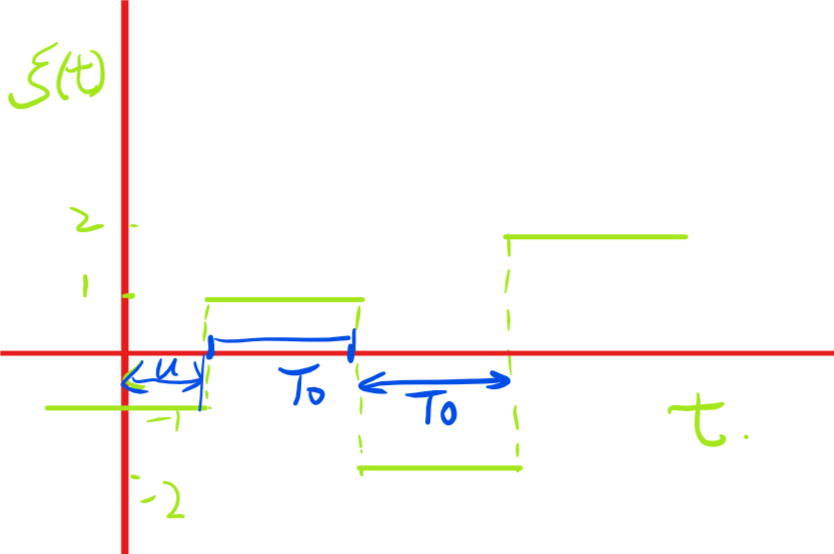
\includegraphics[width=0.6\textwidth]{../../img/math_stochastic/201704191dot2.png}
\caption{\label{fig:orga4a4c7f}
脉冲信号的典型样本函数}
\end{figure}



在时间轴上固定两个时刻\(t_{1},t_{2}\)。首先要研究的问题时\(t_{1},t_{2}\)是否处于一个脉冲内。设事件\(c\)表示\(t_{1},t_{2}\)处于不同的脉冲,它的逆事件\(c^{c}\)表示\(t_{1},t_{2}\)处于同一脉冲周期内。

当\(|t_{1} - t_{2}| > T_{0}\)时,事件\(c\)是必然事件,此时,\(P(c) = 1,P(c^{c}) = 0\),;

当\(|t_{1} - t_{2}| \leq T_{0}\)时,\(t_{1},t_{2}\)有可能在同一脉冲内,也有可能处于两个不同的脉冲内。设\(\theta\)为\(t_{1}\)所在的脉冲的起始时刻。由于脉冲的起始时间相对于原点\(t=0\)的时间差\(u\)均匀分布于\((0,T_{0})\)内,而且该信号为等脉宽的脉冲信号,脉宽均匀为\(T_{0}\)。则\(\theta\)也是均匀分布的随机变量,\(\theta\)可视为均匀分布于\([t_{1}-T_{0},t_{1}]\)内的随机变量。图\ref{fig:orgc9bbe89}给出了\(\theta\)的概率密度和\(t_{1},t_{2},\theta\)的关系图。

\begin{figure}[htbp]
\centering
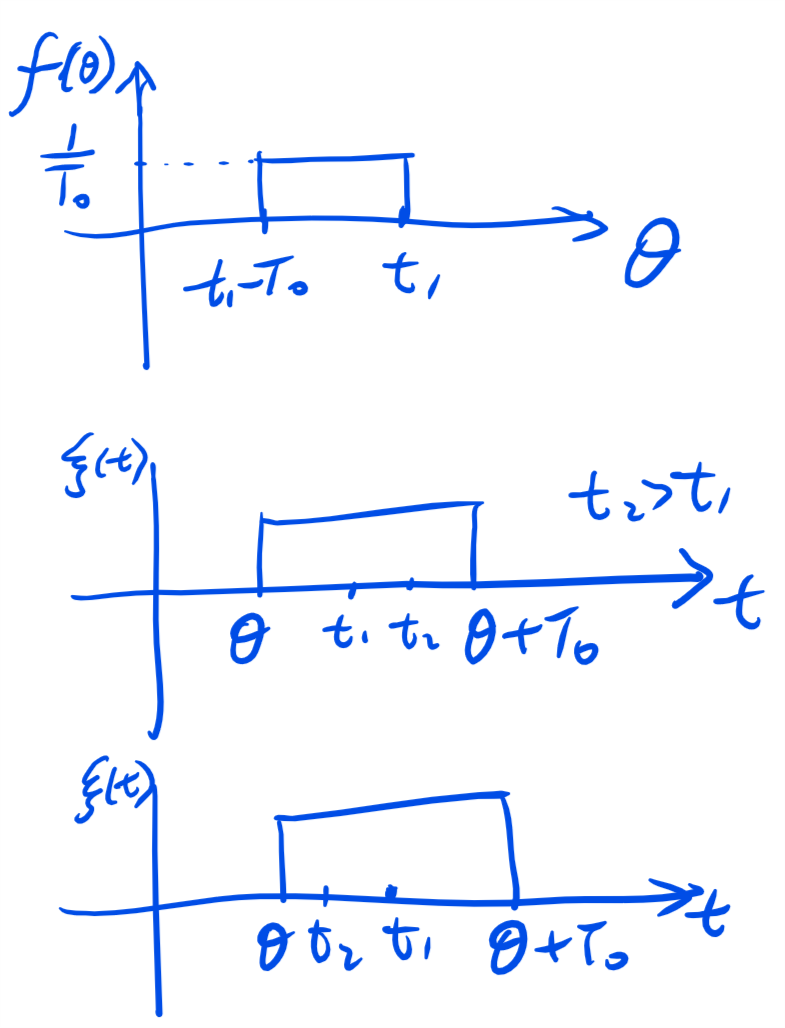
\includegraphics[width=0.6\textwidth]{../../img/math_stochastic/201704191dot3.png}
\caption{\label{fig:orgc9bbe89}
\(t_{1},t_{2},\theta\)关系图}
\end{figure}

如果\(t_{1} < t_{2}\),则:
\begin{eqnarray}
\label{eq:1}
P(c^{c})&=& P(t_{2} < \theta + T_{0}) = P( \theta > t_{2} - T_{0}) \\
&=& 1- P(\theta < t_{2} - T_{0}) \\
&=& 1- \frac{1}{T_{0}}\int_{t_{1} - T_{0}}^{t_{2} - T_{0}} d\theta \\
&=& 1- \frac{t_{2} - t_{1}}{T_{0}}
\end{eqnarray}

如果\(t_{2} < t_{1}\) ,则:
\begin{eqnarray}
\label{eq:2}
P(c^{c})&=& P(t_{2} > \theta) = \frac{1}{T_{0}} \int_{t_{1} - T_{0}}^{t_{2}}d\theta \\
&=& 1- \frac{t_{1}-t_{2}}{T_{0}} 
\end{eqnarray}

因此:
\begin{eqnarray}
\label{eq:3}
P(c^{c})&=&  1- \frac{|t_{1}-t_{2}|}{T_{0}} \\
P(c) &=&\frac{|t_{1}-t_{2}|}{T_{0}}
\end{eqnarray}

根据全概率公式:
\begin{equation}
\label{eq:4}
f_{\xi_{t_{1}},\xi_{t_{2}}}(x_{1},x_{2}) = f_{\xi_{t_{1}},\xi_{t_{2}},c}(x_{1},x_{2}|c)P(c) + f_{\xi_{t_{1}},\xi_{t_{2}},c^{c}}(x_{1},x_{2}|c^{c})P(c^{c}) 
\end{equation}
又因为不同周期内脉冲幅度是相互统计独立的随机变量,于是:
\begin{equation}
\label{eq:5}
f_{\xi_{t_{1}},\xi_{t_{2}},c}(x_{1},x_{2}|c) = \sum_{i=\{-2,-1,1,2\}}\frac{1}{4}\delta(x_{1} - i)  \sum_{k=\{-2,-1,1,2\}}\frac{1}{4}\delta(x_{2} - k) 
\end{equation}

如果\(t_{1},t_{2}\)处于同一周期,则\(\xi(t_{1} = \xi(t_{2}))\),这时:
\begin{equation}
\label{eq:6}
f_{\xi_{t_{1}},\xi_{t_{2}} |c^{c}} = \sum_{i=\{-2,-1,1,2\}} \frac{1}{4}\delta(x_{1} - i)\delta(x_{2} - i)
\end{equation}

综上有:
当\(|t_{1} - t_{2}| \leq T_{0}\)时:

\begin{eqnarray}
\label{eq:9}
f_{\xi_{t_{1}},\xi_{t_{2}}}(x_{1},x_{2}) &=& \sum_{i=\{-2,-1,1,2\}}\frac{1}{4}\delta(x_{1} - i)  \sum_{k=\{-2,-1,1,2\}}\frac{1}{4}\delta(x_{2} - k) \frac{|t_{1} - t_{2}|}{T_{0}}\\ 
&+& \sum_{i=\{-2,-1,1,2\}} \frac{1}{4}\delta(x_{1} - i)\delta(x_{2} - i)(1- \frac{|t_{1} - t_{2}|}{T_{0}})
\end{eqnarray}

当\(|t_{1} - t_{2}| \geq T_{0}\)时:
\begin{equation}
\label{eq:8}
f_{\xi_{t_{1}},\xi_{t_{2}}}(x_{1},x_{2}) = \sum_{i=\{-2,-1,1,2\}}\frac{1}{4}\delta(x_{1} - i)  \sum_{k=\{-2,-1,1,2\}}\frac{1}{4}\delta(x_{2} - k)
\end{equation}
\end{answer}
\end{document}
